
From HW~\ref{ds:pendulum}.5, the linearized equations of motion are given by
\[
\begin{pmatrix} (m_1+m_2) & m_1 \frac{\ell}{2} \\
m_1 \frac{\ell}{2} & m_1 \frac{\ell^2}{4} \end{pmatrix}\begin{pmatrix}
\ddot{\tilde{z}} \\ \ddot{\tilde{\theta}} \end{pmatrix}  =
\begin{pmatrix} -b\dot{\tilde{z}} + \tilde{F} 
	  \\
	m_1 g \frac{\ell}{2} \tilde{\theta} \end{pmatrix}.
\]
Inverting the matrix on the left and side gives
\begin{align*}
\begin{pmatrix}\ddot{\tilde{z}} \\ \ddot{\tilde{\theta}} \end{pmatrix}  
&= \begin{pmatrix} (m_1+m_2) & m_1 \frac{\ell}{2} \\
m_1 \frac{\ell}{2} & m_1 \frac{\ell^2}{4} \end{pmatrix}^{-1}
\begin{pmatrix} -b\dot{\tilde{z}} + \tilde{F} \\m_1 g \frac{\ell}{2} \tilde{\theta} \end{pmatrix} \\
&= \frac{\begin{pmatrix} m_1 \frac{\ell^2}{4} & -m_1 \frac{\ell}{2} \\
-m_1 \frac{\ell}{2} & (m_1+m_2) \end{pmatrix}}{m_1m_2\frac{\ell^2}{4}}
\begin{pmatrix} -b\dot{\tilde{z}} + \tilde{F} \\m_1 g \frac{\ell}{2} \tilde{\theta} \end{pmatrix} \\
&=\begin{pmatrix} -\frac{b}{m_2}\dot{\tilde{z}} + \frac{1}{m_2} \tilde{F} - \frac{m_1g}{m_2}\tilde{\theta} \\ \frac{2b}{m_2\ell}\dot{\tilde{z}}-\frac{2}{m_2\ell}\tilde{F}+\frac{2(m_1+m_2)g}{m_2\ell}\tilde{\theta} \end{pmatrix},
\end{align*}
or in other words, the coupled differential equations
\begin{align*}
\ddot{\tilde{z}} + \frac{b}{m_2}\dot{\tilde{z}} &=  \frac{1}{m_2} \tilde{F} - \frac{m_1g}{m_2}\tilde{\theta} \\
\ddot{\tilde{\theta}} - \frac{2(m_1+m_2)g}{m_2\ell}\tilde{\theta} &= \frac{2b}{m_2\ell}\dot{\tilde{z}}-\frac{2}{m_2\ell}\tilde{F}.
\end{align*}
Taking the Laplace transform with initial conditions set to zero and rearranging gives
\begin{align}
(s^2 + \frac{b}{m_2}s)\tilde{Z}(s) &=  \frac{1}{m_2} \tilde{F}(s) - \frac{m_1g}{m_2}\tilde{\Theta}(s) 
\label{eq:soln_B6_1}\\
(s^2 - \frac{2(m_1+m_2)g}{m_2\ell})\tilde{\Theta}(s) &= \frac{2b}{m_2\ell}s\tilde{Z}(s)-\frac{2}{m_2\ell}\tilde{F}(s).
\label{eq:soln_B6_2}
\end{align}

To find the transfer matrix from $\tilde{F}$ to $(\tilde{Z}, \tilde{\Theta})^\top$, write Equation~\eqref{eq:soln_B6_1} and~\eqref{eq:soln_B6_2} in matrix form as
\[
\left(\begin{array}{c|c}
s^2 + \frac{b}{m_2}s & \frac{m_1g}{m_2} \\\hline -\frac{2b}{m_2\ell}s & s^2 - \frac{2(m_1+m_2)g}{m_2\ell} \end{array}\right)
\begin{pmatrix}\tilde{Z}(s) \\ \tilde{\Theta}(s) \end{pmatrix} 
= \begin{pmatrix} \frac{1}{m_2} \\ -\frac{2}{m_2\ell} \end{pmatrix} \tilde{F}(s),
\]
and invert the matrix on the left hand side to obtain
\[
\begin{pmatrix}\tilde{Z}(s) \\ \tilde{\Theta}(s) \end{pmatrix} 
= \begin{pmatrix} 
\frac{\frac{1}{m_2}s^2-\frac{2g}{m_2\ell}}{s^4+\frac{b}{m_2}s^3-\frac{2(m_1+m_2)g}{m_2\ell}s^2-\frac{2b g}{m_2\ell}s}
\\ 
\frac{-\frac{2}{m_2\ell}s^2}{s^4+\frac{b}{m_2}s^3-\frac{2(m_1+m_2)g}{m_2\ell}s^2-\frac{2 b g}{m_2\ell}s}
\end{pmatrix} \tilde{F}(s).
\]

Plugging in the nominal values from Section~1.\ref{ds:pendulum} we get that there are two fast poles at $2.38$ and $-2.03$, and and two slow poles at 
$0$ and $-0.40$.  Therefore the system is a good candidate for a cascade approximation of fast and slow dynamics.

To find the approximate transfer functions, return to Equations~\eqref{eq:soln_B6_1} and~\eqref{eq:soln_B6_2} and divide by the polynomial on the left hand side to obtain
\begin{align}
\tilde{Z}(s) &=  \frac{\frac{1}{m_2}}{s(s + \frac{b}{m_2})} \tilde{F}(s) + \frac{-\frac{m_1g}{m_2}}{s(s + \frac{b}{m_2})}\tilde{\Theta}(s) 
\label{eq:soln_B6_3}\\
\tilde{\Theta}(s) &= \frac{\frac{2b}{m_2\ell}s}{(s^2 - \frac{2(m_1+m_2)g}{m_2\ell})}\tilde{Z}(s) + \frac{-\frac{2}{m_2\ell}}{(s^2 - \frac{2(m_1+m_2)g}{m_2\ell})}\tilde{F}(s).
\label{eq:soln_B6_4}
\end{align}
Note that the roots of the polynomial $s(s + \frac{b}{m_2})=0$ are at $0$ and $-0.05$, and the roots of the polynomial $s^2 - \frac{2(m_1+m_2)g}{m_2\ell}=0$ are at $\pm 7.0$.  Therefore, Equation~\eqref{eq:soln_B6_3} approximate the slow dynamics and~\eqref{eq:soln_B6_4} approximate the fast dynamics.  Therefore, we let $\tilde{F}$ drive the fast dynamics with output $\tilde{\Theta}$ and we let $\tilde{\Theta}$ drive the slow dynamics with output $\tilde{Z}$.
Since $b$ is small, Equation~\ref{eq:soln_B6_4} can be approximated as
\[
\tilde{\Theta}(s) = \frac{\frac{2b}{m_2\ell}s}{(s^2 - \frac{2(m_1+m_2)g}{m_2\ell})}\tilde{Z}(s) + \frac{-\frac{2}{m_2\ell}}{(s^2 - \frac{2(m_1+m_2)g}{m_2\ell})}\tilde{F}(s),
\]
where $d_2(t)=\mathcal{L}^{-1}\{D_2(s)\}$ is thought of as a small unknown disturbance.  
To find the transfer function from $\tilde{\Theta}$ to $\tilde{Z}$ we note that $\frac{1}{m_2}$ is on the same order of magnitude as $-m_1 g/m_2$, therefore, we cannot simply ignore the first term in Equation~\eqref{eq:soln_B6_3}.  Assuming that the angular dynamics involving $\tilde{\theta}$ have essentially died out, implying that $s^2\tilde{\Theta}\approx 0$ in Equation~\eqref{eq:soln_B6_2} gives
\[
-\frac{2(m_1+m_2)g}{m_2\ell}\tilde{\Theta}(s) \approx \frac{2b}{m_2\ell}s\tilde{Z}(s)-\frac{2}{m_2\ell}\tilde{F}(s).
\]
Therefore
\[
\frac{1}{\ell}\tilde{F}(s) \approx \frac{b}{m_2}s\tilde{Z}(s)
+ \frac{(m_1+m_2)g}{m_2}\tilde{\Theta}(s).
\]
Substituting into Equation~\eqref{eq:soln_B6_1} gives
\begin{align*}
& (s^2 + \frac{b}{m_2}s)\tilde{Z}(s) \approx  
	\frac{b}{m_2}s\tilde{Z}(s)
	+ \frac{(m_1+m_2)g}{m_2}\tilde{\Theta}(s) 
	- \frac{m_1g}{m_2}\tilde{\Theta}(s) \\
\implies & s^2 \tilde{Z}(s) \approx g\tilde{\Theta} \\
\implies & \tilde{Z}(s) = \frac{g}{s^2}\tilde{\Theta} + D_1(s),
\end{align*}
where we assume that $d_1(t)=\mathcal{L}^{-1}\{D_1(s)\}$ is a small unknown disturbances.
The block diagram for the approximate system is shown in Figure~\ref{fig:dm_soln_b6}
\begin{figure}[htbp]
   \centering
   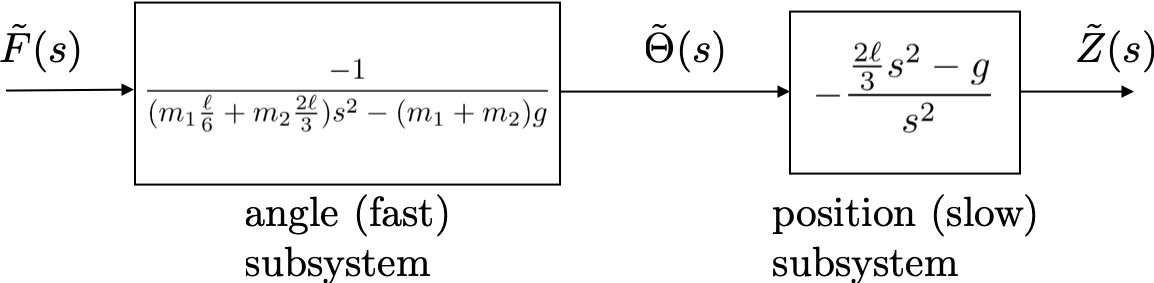
\includegraphics[width=0.8\textwidth]{6_design_studies/figures/hw_pendulum_block_diagram.pdf}
   \caption{The inverted pendulum dynamics are approximated by cascade of fast and slow subsystems.  The fast subsystem is the transfer function from the force to the angle, and the slow subsystem is the transfer function from the angle to the position.}
   \label{fig:dm_soln_b6}
\end{figure}

The cascade approximation makes since physically because the force on the cart has an almost immediate effect on the angle of the rod.  On the other hand, if the angle of the rod is a nonzero constant then the position of the cart must be moving.  Therefore, the desired angle of the rod will dictate a desired velocity for the cart.
